
\subsection{Modelling the experimental data}

In this part the data described in part\,I is interpreted in a physical model and quantitatively formulated in a rate equation scheme.

It is a characteristic feature of the measured current pulse profiles in Fig.~\ref{fig:currentprofiles} that they are rectangular and practically constant a low temperature from 2\,K up to 70\,K at a given electric field. 
Above 70\,K the current amplitudes increase strongly showing rising and falling flanks reminiscent of an $\exp(-t/\tau(T))$-like behaviour with time constants $\tau(T)$ decreasing for higher temperatures. 
Evidently, the current profiles are composed of two different contributions one of which, at increasing temperatures, shows thermal activation.

\begin{figure}[tb]
 \centering
 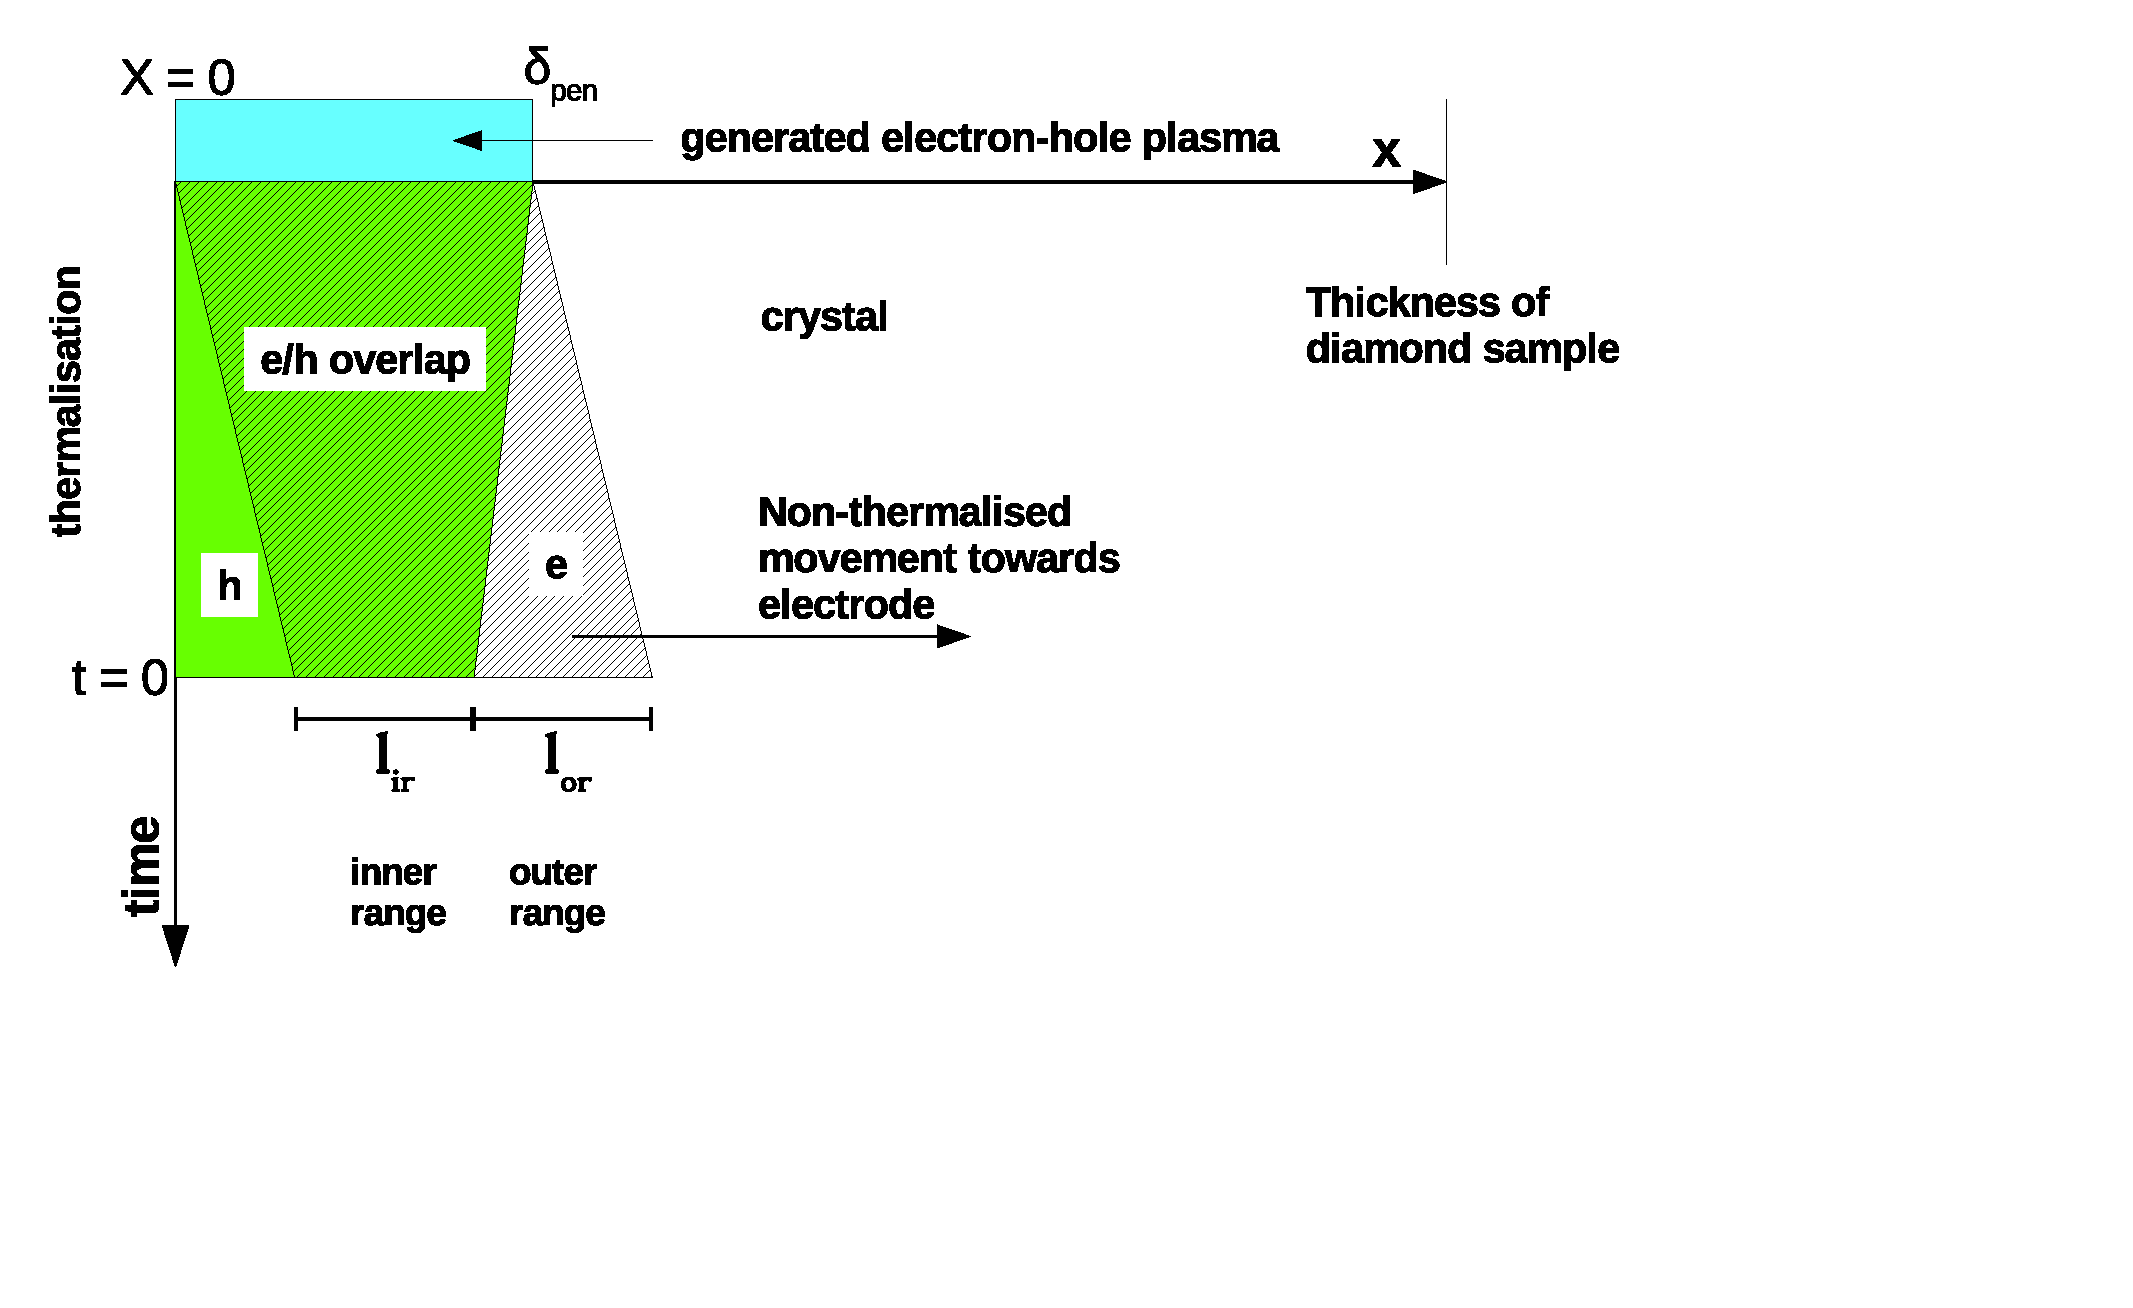
\includegraphics[trim=0 100 250 0, width=0.49\textwidth]{figures/non-therm.eps}\put(-30,30){(A)}
 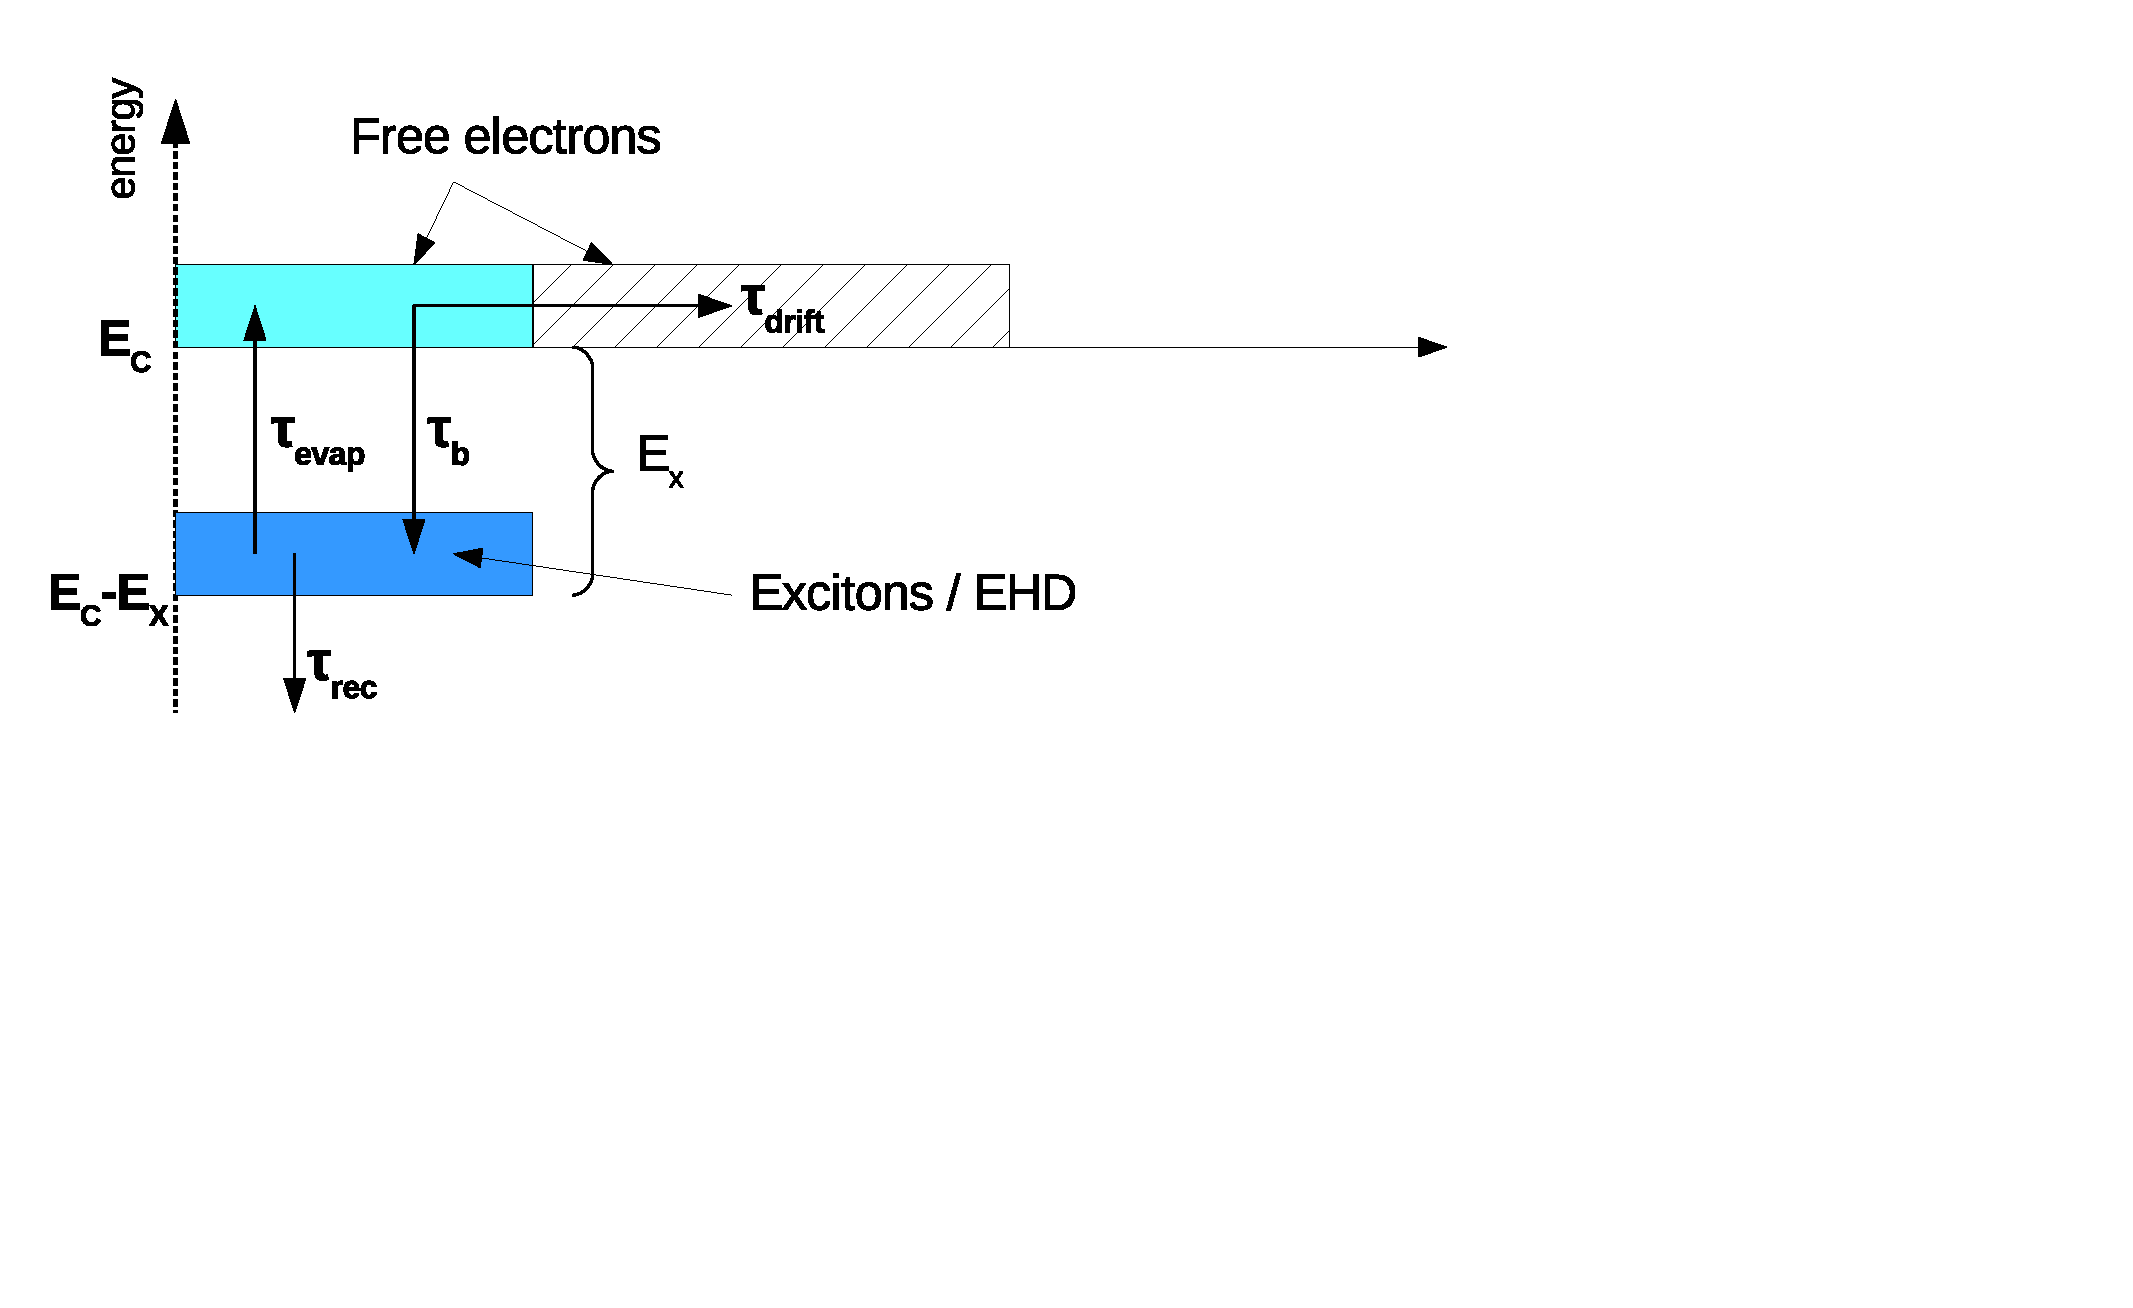
\includegraphics[trim=0 100 250 0, width=0.49\textwidth]{figures/NiveausTaus.eps} \put(-30,30){(B)} \\
 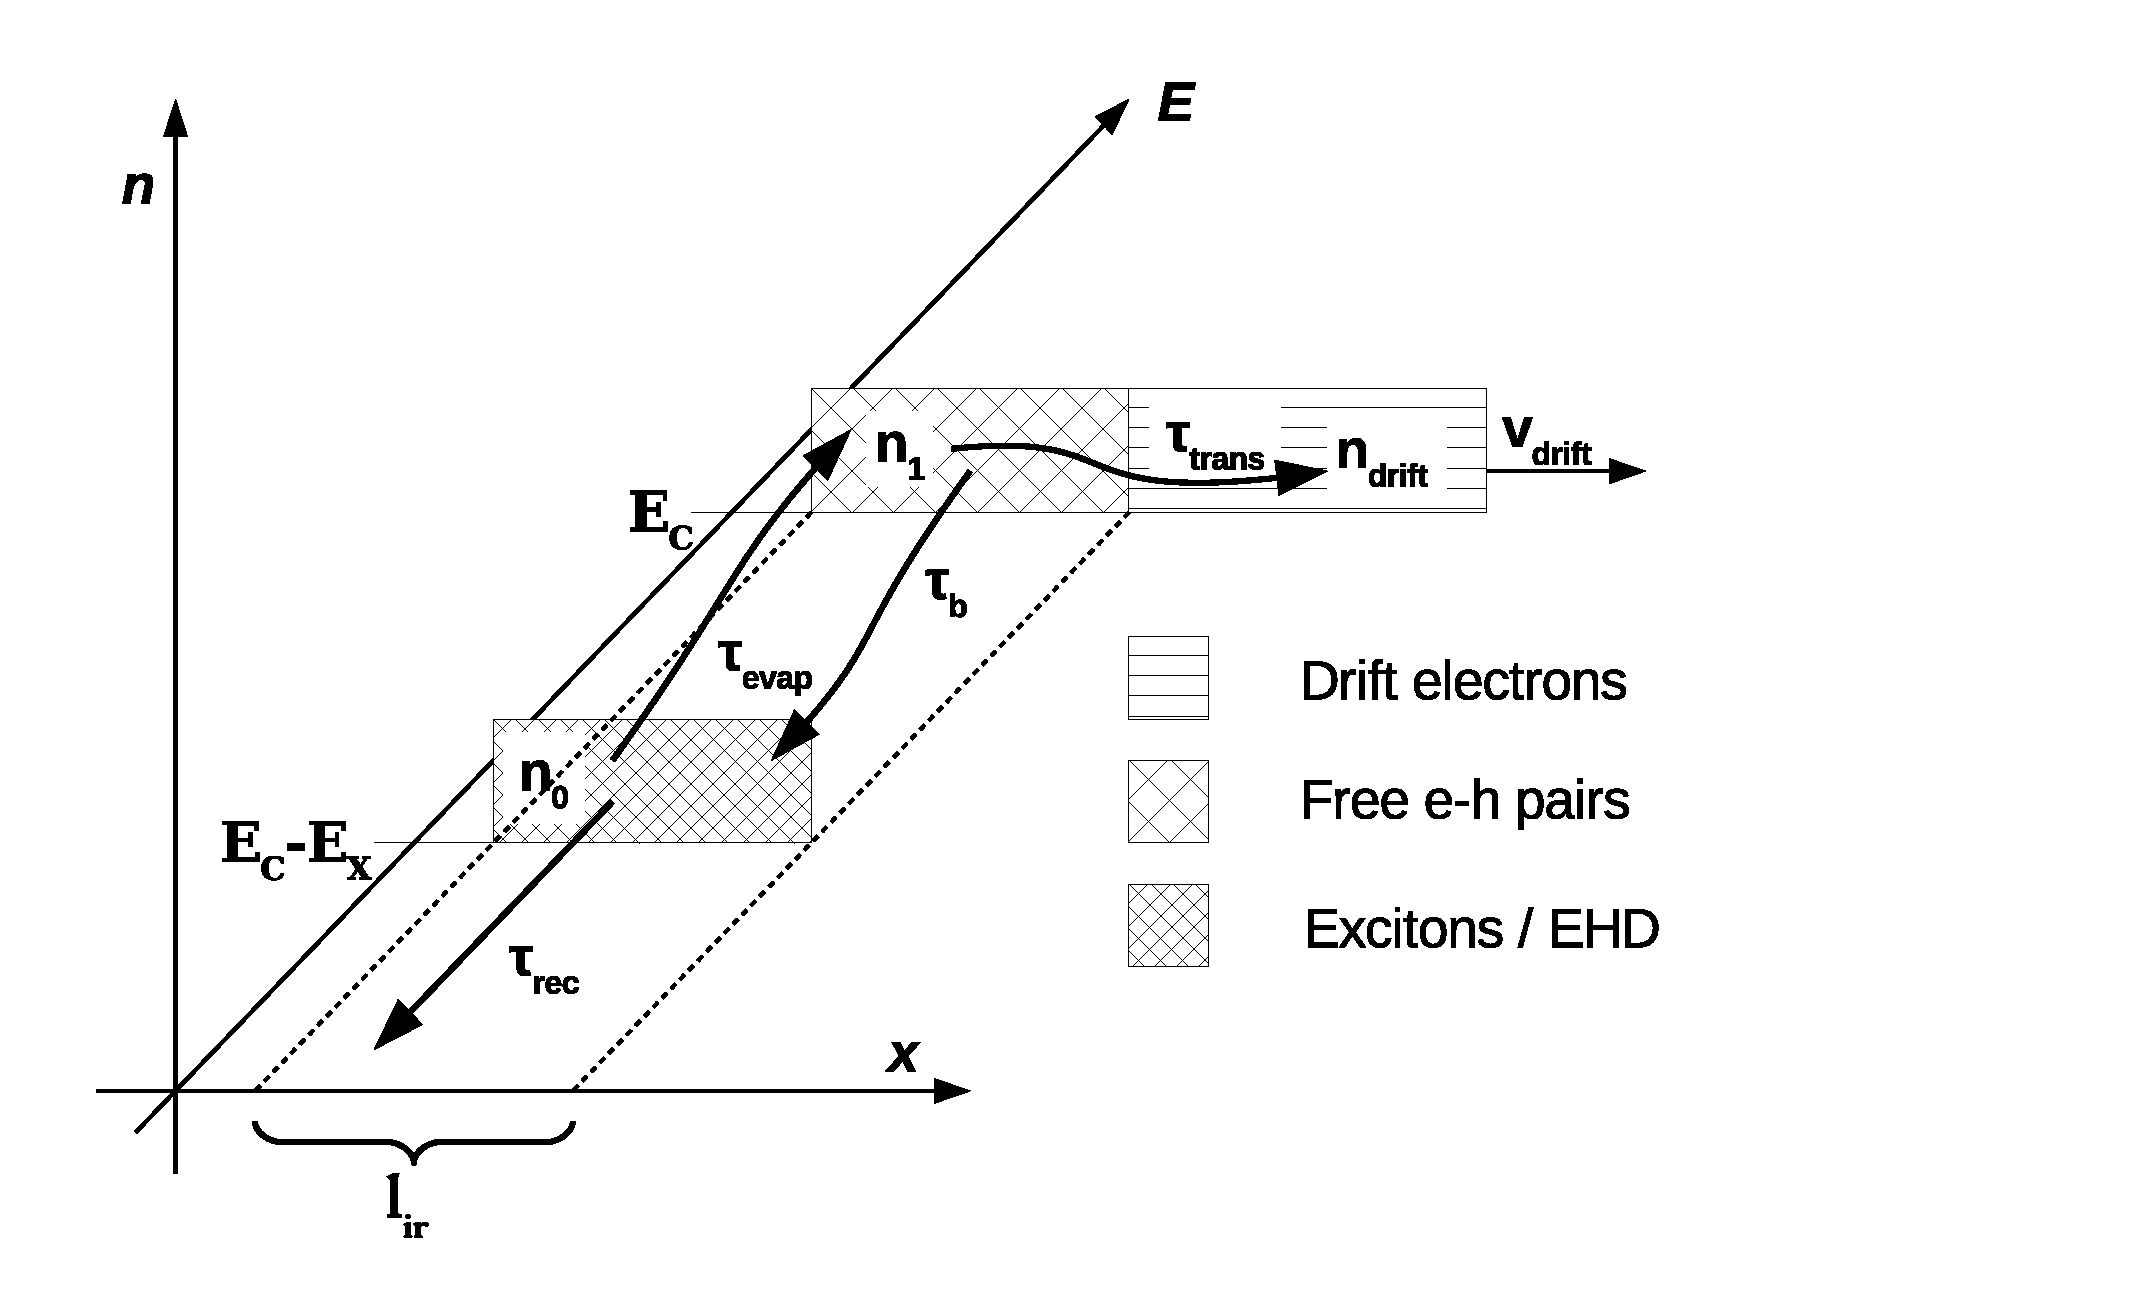
\includegraphics[trim=0  50 100 100, width=0.49\textwidth]{figures/NiveausTaus2.eps}\put(-30,30){(B')}

 \caption{(A) A sketch of the basic idea of the model with an inner and an outer region. 
 (B) The different energy levels and time constants are shown. 
 (B') Vorschlag einer anderen Version von (B), bei der die Dichte und Energie entlang unterschiedlicher Achsen dargestellt sind.}
 \label{fig:non-thermalised}
\end{figure}

The basic idea of the model as sketched in Fig.~\ref{fig:non-thermalised} (A) is the assumption that after the excitation of electrons and holes in highly excited band states
 there is a local separation of the two differently charged species during the relaxation phase under the influence of the electric field: 
 Electrons and holes drift in opposite directions separating locally from each other except for a central range where -  depending on the strength of the electric field  --  they still overlap. 
In this central overlap range, electrons and holes having reached their band edges after relaxation form a bound neutral charge-storage state no longer influenced by the electric field. 
However, this state can be thermally activated to yield a temperature-dependent current contribution. 
This is in contrast to the two outer regions which only contain electrons or holes inducing a temperature independent current. 
In the following, we will call these two ranges the inner and the outer range. 
The model neglects any charge carrier diffusion during relaxation and carrier transit. 
Therefore, it is one-dimensional and carriers move only in the direction perpendicular to the side facets of the $\SI{500}{\um}$ thick samples.

To derive a physical picture of the charge-storage state it is important to note that the temperature and electric field variations of the measured pulse profiles 
 are principally identical for electrons and holes {\color{red}(B1)}. 
We therefore conclude that the bound storage state must involve the two species in totally equivalent roles. 
There are only three types of electron-hole state that satisfy this condition:
 Free excitons (FE), excitons bound to neutral impurities such as donors or acceptors (BE), and electron-hole drops (EHD). 
The experimental part has shown that the activation energy is approximately 80\,meV at the most detailed studied electric field of $\SI{1}{\volt/\um}$ 
 (corresponding to an applied voltage of 500\,V) depending weakly on the electric field {\color{red}(B2)}. 
So, prior to a later more refined discussion, FEs with a binding energy of 80\,meV (Ref.   ) suggest themselves as the bound state in question. 
EHDs have binding energies in excess of the excitonic binding of 52...58\,meV (Ref.    ) significantly too much at the present status of the discussion {\color{red}(B3)}. 
BEs can definitely be excluded from further discussion: There is only one typical shallow impurity in diamond, the acceptor boron binding a hole with an ionization energy of\,370 meV. 
In this this neutral state boron can localize a FE with 55\,meV into a BE state. 
Though all diamonds contain small amounts of boron (often only detectable by sensitive luminescence analysis) our samples are yellowish indicating dominant doping with nitrogen,
 and the amount of boron would be far too low to govern the observed characteristic storage behaviour in which high carrier concentration up to $\SI{1e18}{\cm^{-3}}$ are involved. {\color{red}(B4)}
 

\subsubsection{Outer range}

For definiteness we discuss here the situation with electrons; holes can be treated completely analogously with parameter changes \textit{mutatis mutandis}.
The electron concentration in the outer range at the end of the relaxation phase is called $\No(0)$. 
The resulting current measured at the anode is

\begin{equation}
 j(t) = q\No(0)v(t)\quad {\color{red}(B5)}. 
\end{equation}

\noindent
The electron package reaches the anode at the transit time $t'$, from then the current decreases linearly to zero in a time interval of  $\Delta t = \dpen/v$  since the incoming carriers flow into the anode. 
Here $\dpen$ is the length of the initial ionisation volume at $t = 0$ (Fig.~\ref{fig:non-thermalised} (C)) and $v$ the applicable carrier velocity. 
Referring to the later discussion of possible values for these parameters we expect $\Delta t$ to lie in the picosecond range. 
This is too short to be experimentally resolved. 
The measured pulse profile is then simply rectangular with a duration of $\SI{500}{\um/v}$ and smeared edges due to scattering effects during the transit. 
For holes also rectangular current pulse profiles are measured and explained analogously.

\subsubsection{Inner range}

In the inner range the situation developed so far is modelled by a set of coupled rate equations following the intuitive sketch in Fig.~\ref{fig:non-thermalised}~(C). 
Prior to the formulation of the equations we describe the model in physical terms, referring to electrons in order to be specific.

The concentration of electrons bound in excitons in the inner range does not contribute to the measured current at low temperatures until the excitons are thermally dissociated at increasing temperatures. 
In the bound state, the electron concentration is denoted as $n_0$ and the electrons have an energy of -80\,meV relative to the conduction band edge at $\Ec = 0 $. 
During the excitonic binding, recombination can take place. 
We note in passing that even our highest fields are not able to tear off the excitons as a simple estimate shows. 
In the activated state, the electrons with concentration $n_1$ are free at energy $\Ec = 0 $ and can be extracted from the inner range by the electric field.
With these partial processes the rate equations read as 

\begin{align}
\label{math:diff1}
 \frac{\dd n_1}{\dd t} &= -\frac{n_1}{\tauone}  + \frac{n_0}{\tauevap} \qquad \textrm{with} \qquad\frac{1}{\tauone} = \frac{1}{\taub} + \frac{1}{\taudrift} \quad {\color{red}(B6)}\\
 \frac{\dd n_0}{\dd t} &= -\frac{n_0}{\tauzero} + \frac{n_1}{\taub} \qquad \textrm{with}    \qquad\frac{1}{\tauzero}= \frac{1}{\tauevap} + \frac{1}{\taurec} \quad {\color{red}(B7)}
 \label{math:diff2}
\end{align}

\noindent
The time constants are

\begin{itemize}
 \item $\tauone$: dwell time of $n_1$-electrons given by the competing loss processes of binding into excitons ($\taub$) and drift out of the inner range due to the electric field ($\taudrift$).
 \item $\tauzero$: lifetime of $n_0$-electrons (excitons)  given by the competing processes of exciton dissociation (or evaporation, $\tauevap$) and exciton recombination ($\taurec$).
\end{itemize}

\noindent
The drift time $\taudrift$ may be set equal to the extraction or depletion time of the inner range with extension $\lir$ as $\taudrift  = \lir/2v$,
 where the drift velocity $v$ depends on temperature and electric field. 

The set of rate equations (\ref{math:diff1}) and (\ref{math:diff2}) cannot be solved analytically. 
However, a simplification is possible so as to open a way for an analytical solution. 
The time $\taub$ describing the binding of $n_1$ electrons into excitons  may be expressed in the form

\begin{equation}
 \taub = 1/(\sigma \vth n_1) 
\end{equation}

\noindent
where $\sigma$ denotes the capture cross section for the binding into excitons, and $\vth$ is the average thermal velocity of the electrons. 
$\sigma$ can be calculated from the Bohr radius $r_x$ of the excitons, $\sigma  = 4 \pi {r_x}^2$  yielding with  $r_x = \SI{1.4}{\nm}$  as discussed in (Ref......)  a value $\sigma  \approx \SI{6e-14}{\cm^2}$,
 and $\vth = \sqrt{3\kB T/m\cdot\e }= \SI{1e7}{\cm/\s}$ at room temperature. 
Directly after relaxation, with an initial electron concentration of $n_1(0) = \SI{1e18}{\cm^{-3}}$ as estimated in the experimental part, $\taub$ is around 1.6\,ps,
 much shorter than $\tauevap = 1.2 \cdot \exp{80\,meV/\kB T}$ {\color{red}(B8)}.
The latter expression was derived from the experimental data:
 At high temperatures, $T \approx \SI{170}{\kelvin}$, it merges below 200\,ps, the experimental limit of resolution;
 at low temperatures, $T \approx \SI{100}{\kelvin}$, it goes over into the time constant $\taurec \approx  \SI{10}{\ns}$ of the competing parallel process of recombination. 
Hence, directly after exciton formation, $n_0(0) \gg   n_1(0)$ and $n_0(0) = \Nin(0)$ is practically equal to the whole inner electron concentration $\Nin(0)$. 

These considerations lead to the simplified equations

\begin{align}
\label{math:diff3}
 \frac{\dd n_1}{\dd t} &= -\frac{n_1}{\taudrift}  + \frac{n_0}{\tauevap},\quad {\color{red}(B9)}\\
 \frac{\dd n_0}{\dd t} &= -\frac{n_0}{\tauzero}.
 \label{math:diff4}
\end{align}

\noindent
The solution of (\ref{math:diff4}) is straight forward

\begin{equation}
 n_0(t) = n_0(0)\cdot \exp{\left(-t/\tauzero\right)}. 
\end{equation}

\noindent
The solution of (\ref{math:diff3}) is obtained as the solution of the homogeneous equation plus one particular solution of the inhomogeneous equation yielding

\begin{equation}
 n_1(t) = \left[ n_1(0) - \frac{\tauzero\taudrift}{\tauevap(\tauzero-\taudrift)} n_0(0)\right]\cdot \exp{\left(-t/\taudrift\right)} 
                        + \frac{\tauzero\taudrift}{\tauevap(\tauzero-\taudrift)} n_0(0) \cdot \exp{\left(-t/\tauzero\right)}
  \label{math:sol1}
\end{equation}

\noindent
The depletion of the inner range by electron drift is according to equation (\ref{math:diff3})

\begin{equation}
 \frac{\dd n_1}{\dd t}{}_{\big|_{\drift}} = + \frac{n_1(t)}{\taudrift} \equiv \frac{\dd \ndrift (t)}{\dd t}
\end{equation}

Here, the positive sign has to be taken as we are concerned with the electron concentration on the drift stretch lacking in the inner range.
The current released from the inner range to the drift stretch after integration of $\ndrift$ becomes {\color{red}(B10)}

\begin{equation}
 j(t) = \q \ndrift(t) v(t) = \q v(t) n_0(0) \cdot \frac{\tauzero}{\tauevap(\tauzero-\taudrift)} \cdot \Big[ -\taudrift\big( 1- \exp{(-t/\taudrift)}\big) + \tauzero\big( 1 - \exp{(t/\tauzero)} \big) \Big],
\end{equation}

\noindent
where $n_1(0) \ll n_0(0)$ has been neglected. 
$\taudrift = \lir/(2v)$ takes values from 67\,ps to 170\,ps for typical electric fields of $\SI{1.4}{\volt/\um}$ to $\SI{0.2}{\volt/\um}$, respectively. 
$\tauevap$ in comparison is much larger for $T \leq \SI{200}{\kelvin}$. 
These values of $\tauevap$ are not essentially changed when recombination times of the order of a few nanoseconds are included in $\tauevap$. 
Therefore, the first term in the brackets can be neglected yielding an approximate drift current of {\color{red}(B11)}

\begin{equation}
 j(t) =  \q n_1(0)v(t) \frac{\tauzero^2}{\tauevap(\tauzero-\taudrift)} \big( 1- \exp{(-t/\tauzero)}\big).
\end{equation}

This is in fact the pulse profile which we measure as the temperature-activated current contribution. 
The rising flank in the experiments corresponds to the term in brackets, and the asymptotic current value reflects complete electron depletion of the inner range. 
The pre-factor containing various time constants has the character of a supply efficiency limiting the current subject to the recombination time. 
When all restrictions of the time constants apply which were discussed, the pre-factor simplifies to unity. 
The falling flank of the pulse is given by an exponential $\exp(-t/\tau(T))$ as experimentally observed.

The total {\color{red}(B12)} incoming charge $Q$ measured at the anode is the integral of the drift current from $t = 0$ to $t= t'$

\begin{align}
 \Qin &= \q v \Nin(0) \frac{\tauzero^2}{\tauevap(\tauzero-\taudrift)} \cdot \Big[ t' - \tauzero \big( 1- \exp{(-t'/\tauzero)}\big) \Big] \\
   &= \q \Nin(0) \frac{\tauzero^2}{\tauevap(\tauzero-\taudrift)} \Big[  \SI{500}{\um} - v\tauzero \big( 1- \exp{(-t'/\tauzero)}\big) \Big] {\color{red}(B13)}
\end{align}

\noindent
and for $t = 0$ to $t = \infty$ (a few time constants) [jetzt mit $1/d$]

\begin{align}
 \Qin &= \q v/d \cdot \Nin(0) \frac{\tauzero^2}{\tauevap(\tauzero-\taudrift)} \cdot \Big[ t' \Big] \\
   &= \q \Nin(0) \frac{\tauzero^2}{\tauevap(\tauzero-\taudrift)}
\end{align}

\noindent
after insertion of the transit time $t´ =  \SI{500}{\um/v}$.
The first term in brackets, together with the pre-factors,
 corresponds to the total charge which was initially in the inner range and is entirely extracted for high enough temperatures to activate all electrons from there. 
The second term describes the loss out of the total charge due to those electrons which were not thermally activated at low temperatures remaining in the inner range and finally recombining there. 

\subsubsection{Total charge {\color{red}(B14)}}
Combining the inner and the outer currents and integrating to $t = t'$, we obtain

\begin{align}
 \Qtot &= \Qo(0) + Q_1(0) + Q_0(0) \frac{\tauzero}{\tauevap}\left[ 1 - \frac{\tauzero}{t'}(1 - \exp(-t'/\tauzero)) \right]\\ 
 &\approx \Qo(0) + \Qin(0) \frac{\tauzero}{\tauevap}\left[ 1 - \frac{\tauzero}{t'}(1 - \exp(-t'/\tauzero)) \right]
 \label{math:Q}
\end{align}

\noindent
and again for integration to $t = \infty$
\begin{equation}
 \Qtot = \Qo(0) + Q_1(0) + Q_0(0) \frac{\tauzero}{\tauevap}.
\end{equation}

\noindent
Assuming $Q_1(0)$ to be negligible and hence $Q_0(0) \approx \Qin(0)$, we obtain

\begin{equation}
 \Qtot = \Qo(0) + \Qin \frac{\tauzero}{\tauevap} = \Qo(0) + \Qin(0) \frac{1}{1+\frac{\tauevap}{\taurec}} = \Qo(0) + \Qin(0) \frac{1}{1+\frac{t_{e,0}}{\taurec}\cdot \exppEa}. 
 \label{math:Q2}
\end{equation}

\noindent
The expressions (\ref{math:Q}) and (\ref{math:Q2}) were used in Fig.~\ref{fig:QT} to fit the experimentally measured charge at the electrode, cf.\ also Eqs.~)\ref{eq:fitQinfty}) and ~(\ref{eq:fitQtprime}),
 and the agreement is very satisfactory for both electrons and holes. 


\subsection{Dependence of the activation energy $\Ea$ on the electric field}

Most of the experiments were initially performed at an electric field  $\xi = \SI{1}{\volt/\um}$ (applied voltage 500\,V) yielding an ample set of data points for $Q(T)$, c.f.\ Fig.~\ref{fig:QT}. 
In the course of the work $Q(T)$ was also measured for other field strengths extending from $\SI{0.2}{\volt/\um}$ (voltage 100\,V) to $\SI{1.8}{\volt/\um}$ (voltage 900\,V). 
Fits of eq. (\ref{math:Q}) {\color{red}(B15)} to these cases showed that the thermal activation energy $\Ea$ depends on $\xi$, decreasing weakly for $\xi \geq \SI{1}{\volt/\um}$
 and increasing in succession more strongly towards lower field strengths, cf.\ Fig.~\ref{fig:Eafield}. 
This result casts doubts on our initial conclusion that the charge storage state in the inner range consists of FEs {\color{red}(B16)}. 
An approximate free-hand extrapolation to $\xi = 0$ yields a value of $\Ea$ between 125\,meV and 140\,meV.

\begin{figure}[tb]
 \centering
 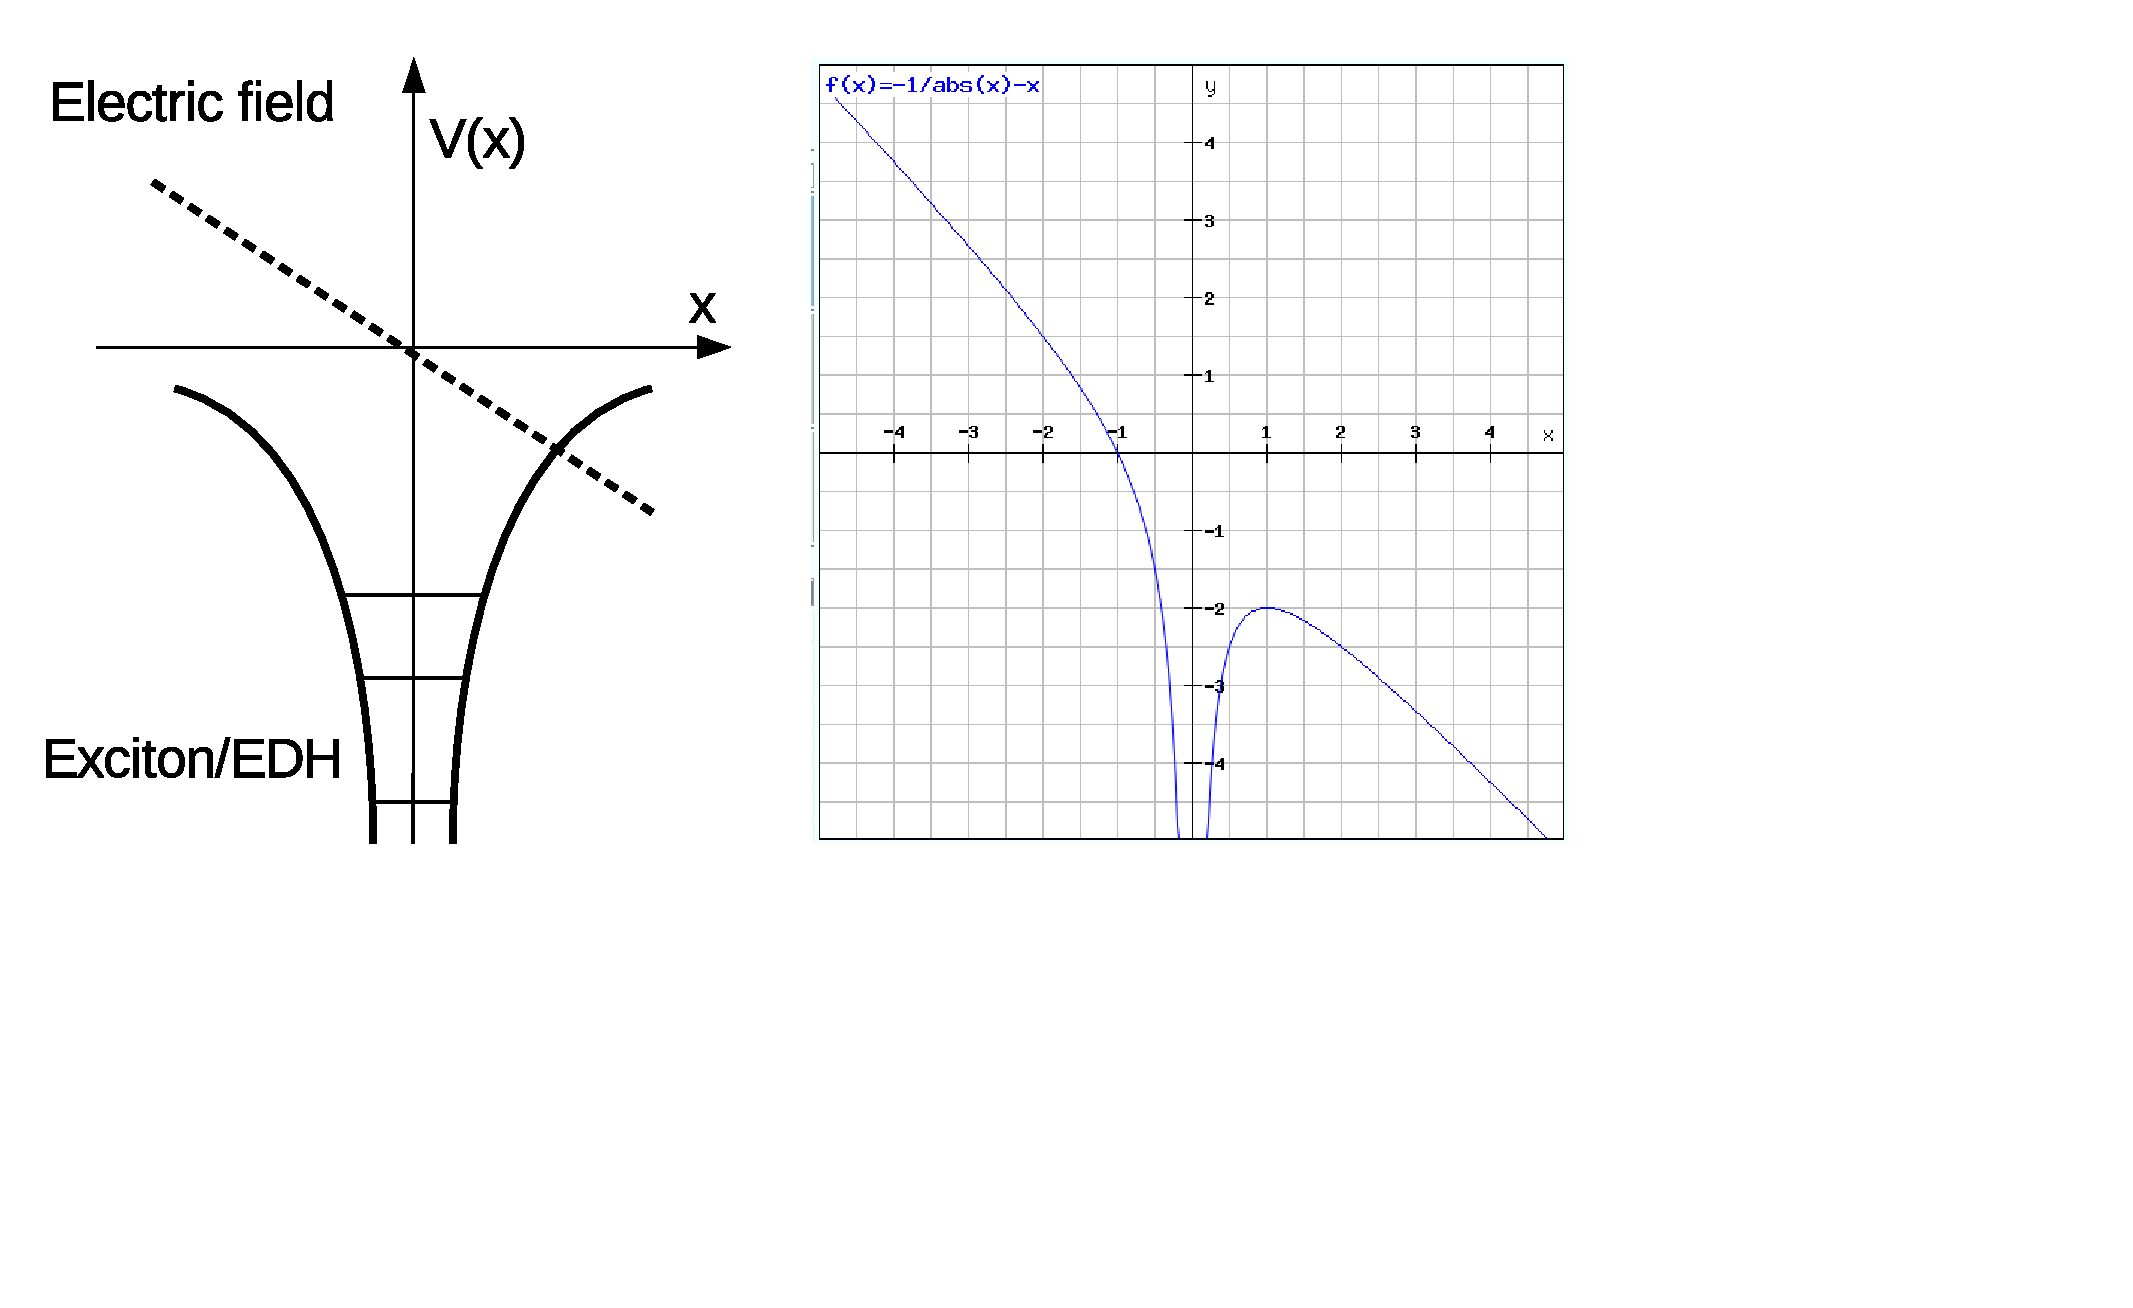
\includegraphics[trim=0 170 0 0, width=0.8\textwidth]{figures/ExcField.eps}
 \caption{(A) The electric potential for a FE and the externally applied voltage are shown separately. (B) The combination of a linearly decreasing field with a hydrogenic potential of the FE. 
 [Fuer rechts zeichne ich noch ein schoeneres Bild.]}
 \label{fig:excfield}
\end{figure} 

As discussed earlier, defects if considered as storage states must bind electrons and holes in an equivalent way. 
Above, we have argued that boron, the only shallow and typical impurity in diamond, must be discarded as a centre to bind FEs into BEs. 
The only alternative satisfying the condition of equivalent electron-hole binding are EHDs. 
In EHDs the additional electron-hole binding in excess of the FE binding amounts to 52...58\,meV (Ref.     ) so that a total binding energy of
 $\Ea = (80 + 52..58)\,\si{\milli\eV}$ would result in good agreement with our rough estimate. 
The phase diagram of FE gas and EHD liquid has been studied recently in detail, and it has been found that the critical temperature $\Tc$ up to which EHDs can exist is 173\,K. 
At this temperature, in our experiments nearly all electrons from the storage state have been thermally dissociated. 
We conclude that for the whole temperature range in the electron charge collection measurements {\color{red}(B17)} one unique activation energy $\Ea$ does apply. 
Also, none of the restrictions made in the deduction of the expressions (9) above is violated by invoking EHDs in addition to FEs  in the activation process.

(Der Absatz ist m.M.n.\ wichtig, um zu argumentieren, dass die Aktivierungsenergie durchaus mehr als 80\,meV sein kann. Deswegen wuerde ich den Absatz beibehalten.)
It remains to be discussed whether the excitation is strong enough to create EHDs. 
The original excitation strength by the incoming $\alpha$-particles is very high amounting to $\SI{1e21}{\cm^{-3}}$ e-h pairs in a pulse {\color{red}(B18)}. 
Following literature data, it might be assumed that the charge carriers do not slowly diffuse but are pushed away from the excitation region by the phonons which they create in their relaxation
 from the high-energy states down to the conduction or valence band edges, respectively. 
In the literature, this driving force is called phonon wind (Ref.   ). 
A simple estimate not reported here shows that – if the phonons would travel isotropically in space from their excitation region
 -- the e-h concentration would decrease dramatically within a relaxation time of 0.1 to 1 ps down to a value where no EHD formation is possible. 
However, it is well known (Ref.        ) that the phonons travel in anisotropic,
 strongly focused channels creating a phonon caustic due to the fact that the directions of their $k$-vectors and their energy flow are not collinear. 
The generated e-h plasma is thought to be driven in such narrow local channels during the relaxation process, that the electrons are strongly scattered out of the channels by carrier-carrier interaction
 and impurity-assisted scattering so that their concentration after relaxation would be by far sufficiently high to condensate into EHDs.

\begin{figure}[tb]
 \centering
 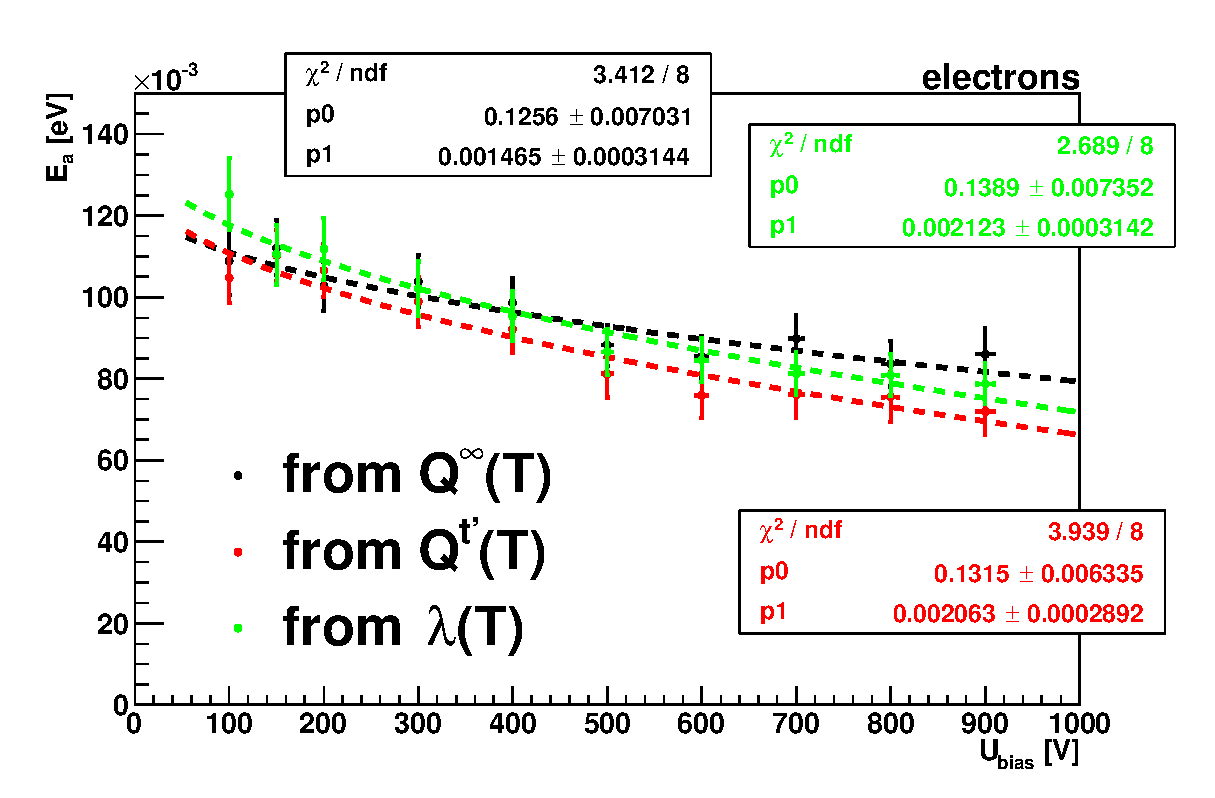
\includegraphics[trim=0 0 0 0, width=0.49\textwidth]{figures/EaU_e.eps}
 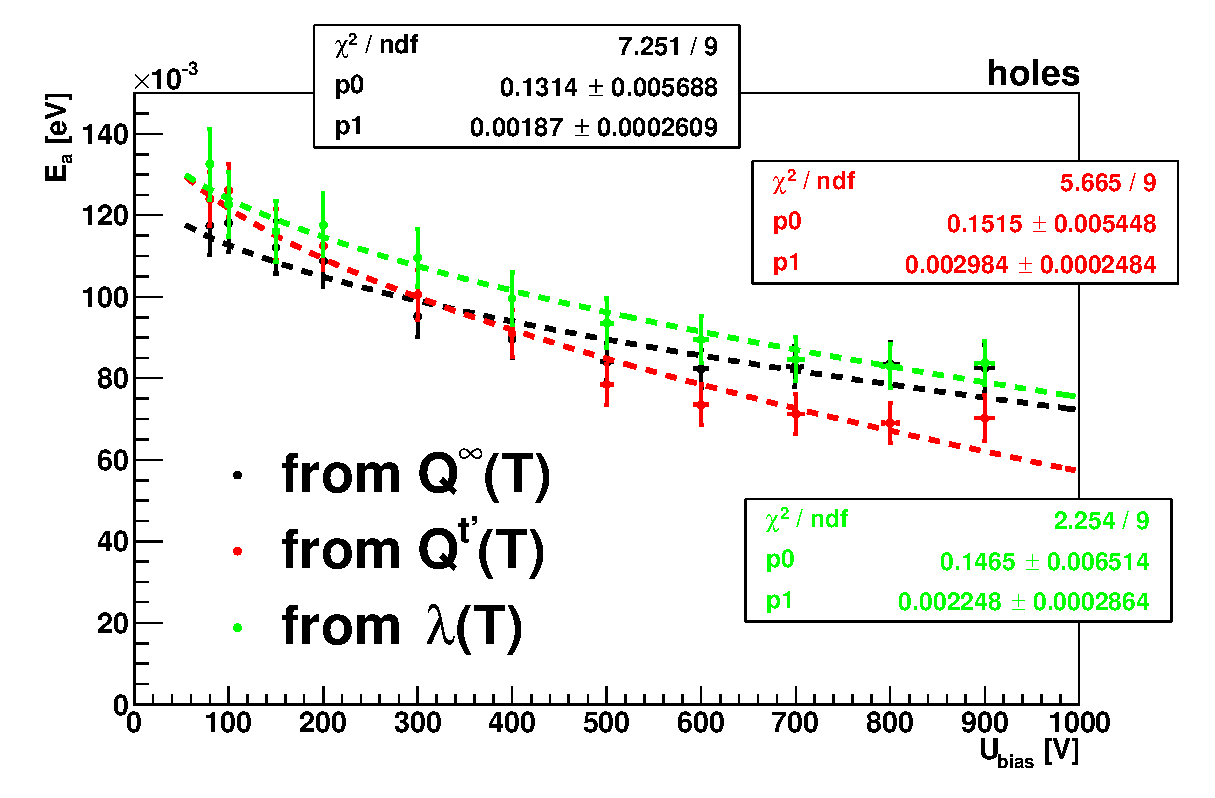
\includegraphics[trim=0 0 0 0, width=0.49\textwidth]{figures/EaU_h.eps}
 \caption{The activation energy as obtained from $Q(T,E)$ and $\lambda(T,E)$ are plotted as a function of the electric field. 
 Fit-functions are overlaid and discussed in section~\ref{sec:discussion}. [Anm.: Die Statistikboxen kommen spaeter noch weg oder werden schoener gemacht.]}
 \label{fig:Eafield}
\end{figure} 

To come to a quantitative expression for $\Ea(\xi)$, we discuss the e-h binding potential in an electric field (Fig.\ref{fig:excfield}). 
The sum of the excitonic Coulomb potential, $V = -\e^2 / (4\pi\varepsilon\varepsilon_0 x)$ and the superposed electric field potential, $V = -\e\xi x$ is asymmetric
 with a local maximum at $x_{\textrm{max}} = \e / \sqrt{4\pi\varepsilon\varepsilon_0 \xi}$ {\color{red}(B18')}
 lowered in comparison to the ionization limit of FEs by $\Delta E(x_{\textrm{max}}) = -2\e^2 ( \xi / \sqrt{4\pi\varepsilon\varepsilon_0 \e} )$. 
This reduces the ionization energy of the FEs {\color{red}(B19)} to a value 
 
\begin{equation}
 \Ea(\xi) = \Ea(0) - \Delta E(\xi) = \Ea(0) - \e\cdot \frac{2\e}{ \sqrt{4\pi\varepsilon\varepsilon_0 \e d} } \cdot\sqrt{U}
 \label{math:delta}
\end{equation}

\noindent
The pre-factor $\frac{2\e}{ \sqrt{4\pi\varepsilon\varepsilon_0 \e d} } = \SI{1.4e-3}{\sqrt{\volt}}$ can be compared to a fit of the form $\Ea - C\cdot\sqrt{U}$,
 resulting in pre-factors of about $\SI{2.0(3)}{\sqrt{\volt}}$, which is in reasonable agreement with the model. 

The envelope function of FEs is hydrogen-like having s-like even symmetry. 
Therefore, the envelope function will not cause any splitting or shift in the electric field of p-like odd symmetry.
However, there are additional non-hydrogenic degrees of freedom in the FEs:
 The electron $\Gamma6$ state splits twofold  in an electric field due to the lifting of the orientational degeneracy (“valley-orbit splitting”), and the hole $\Gamma8$ state also splits into two. 
The total fourfold splitting cannot quantitatively be calculated due to the lack of values for the electric compliance constants. 
We estimate, however, that in diamond these effects are negligible even at our highest fields of $\SI{1.8}{\volt/\um}$ not exceeding a few meV.
Fits to the experimental activation energies in Fig.~\ref{fig:Eafield} have been made using eq.\ (\ref{math:delta}) with $\Ea(0)$ as a free fit parameter. 
Results are presented superimposed on the experimental data in Fig.~\ref{fig:Eafield} showing good agreement for $\Ea(0) = \SI{130}{\milli\eV}$. 
This value is fully compatible with a binding energy of (80 + 52..58)\,meV for EHDs being the storage state in our experiments.



\subsection{Dependence of the collected charge on the electric field}

\subsubsection{Low-temperature case}

At low temperature, $T = \SI{2}{\kelvin}$, the collected charge is exclusively provided by the outer range. 
The data points lie well on a straight line up to the highest field value $\xi = \SI{1.8}{\volt/\um}$, cf.~Fig.~\ref{fig:QvsE}. 
This applies analogously to holes. 
In the model, the electron concentration available for the drift at t = 0 in the outer range depends on the electric field which has separated electrons and holes during the relaxation. 
If the drift velocities in this process are independent of the electric field (in contrast to the band edge velocities)
 the extension of the outer range $x_\e$ would be linear as a function of the field and with it the electron concentration and the collected charge. 
As mentioned at the outset of the paper (SOLLTE AM ANFANG VON PART II ERWAEHNT WERDEN), no literature data on drift velocities in highly excited electron or hole states have been found to document this case. 
Extrapolation of our data points to higher fields delivers an intersection with the curve for the total collected charge measured at $T = \SI{295}{\kelvin}$ at $\xi = \SI{4.5}{\volt/\um}$. 
In the model, this hypothetical value characterizes the case where electrons and holes have been completely separated by the field in the relaxation process leaving no inner overlap range,
 hence $x_\e + x_\h = \SI{10}{\um}$. 
Assuming in this crude estimate equal velocities for electrons and holes, we have $x_\e = \SI{5}{\um} = \vrelax \taurelax$. 
For an assumed relaxation time of $\taurelax$ in the order of 0.1\,ns a drift velocity of $\SI{5e6}{\cm/\s}$ follows comparable to the range of drift values at the band edges at medium fields. 
This gives us confidence that the model also in this respect is physically realistic although it cannot be further documented.

\subsubsection{High-temperature case}

{\color{red}(B28')}
We discuss the data for the highest experimental temperature, $T = \SI{295}{\kelvin}$, and low electric fields. 
This case is not covered by the rate equations since $\tauevap \leq \taudrift$, and electrons thermally activated from $n_0$ are not totally extracted from the inner range. 
Therefore, $n_1$ increases and the earlier made simplifications are no longer valid. 
However, a different approach can be made to describe the collected charge in this case.
When $n_1$ increases, $\taub$ decreases by virtue of $\taub = 1/ (\sigma \vth n_1)$ leading to a quasi-equilibrium of $n_1$ and $n_0$,
 since the loss processes drift ($\taudrift$) and recombination ($\taurec$) are only small in comparison to the carrier re-distribution rates given by $\taub$ and $\tauevap$. 
It is then irrelevant which of the two states suffers the loss. 
We may define a “charge collection efficiency” as the ratio of the desired drift rate to the total loss rate

\begin{equation}
 Q / Q_0 = R_\drift / (R_\drift + R_\textrm{rec}) = \frac{1/\taudrift}{1/\taudrift + 1/\taurec} = \frac{\taurec}{\taurec + \taudrift}.
\end{equation}

\noindent
With $\taudrift = \lir/2v = \lir/2\mu_\e\xi$ we obtain

\begin{equation}
 Q(\xi) / Q_0 = \frac{2\mu_\e \xi \taurec}{l + 2\mu_\e\xi\taurec}.
\end{equation}

\noindent
Low-field values for $\mu_\e$ are contained in the figures...  of (Ref. {\color{red}(B29)}), $\mu_\e = \SI{1150}{\cm^2/\volt\s}$, and $l = \SI{10}{\um}$ so that 

\begin{equation}
 Q(\xi) / Q_0 = \SI{2300}{\cm^2/\volt\s} \xi \taurec / \left( \SI{10}{\um} + \SI{2300}{\cm^2/\volt\s} \xi \taurec \right).
\end{equation}

\noindent
This expression describes approximately the observed drop of $Q(\xi)$ for $T = \SI{295}{\kelvin}$ and low fields for a recombination time close to $\taurec = \SI{14}{\ns}$.

% \subsection{Recombination time}
% The recombination time can be readily extracted from data for temperatures between 100 and 125\,K.


\subsection{Valley re-population effects}

The transit time $\ttr$ of electrons was measured versus temperature for electric fields from
 $\xi = \SI{0.08}{\volt/\um}$ (applied voltage 40\,V) to $\xi = \SI{1.8}{\volt/\um}$ (applied voltage 900\,V) (Fig.~\ref{fig:tt}). 
At high fields $\ttr$ is small and constant up to 100\,K, and then increases due to electron scattering by phonons. 
The transit time is larger for lower applied voltages and, beginning at 300\,V, successively more pronounced maxima for voltages down to 40\,V are observed
 which appear systematically shifted towards lower temperatures. 
We ascribe this effect to a 'valley re-population' between ``fast'' and ``slow'' electrons in the electric field. 

\begin{figure}[tb]
 \centering
 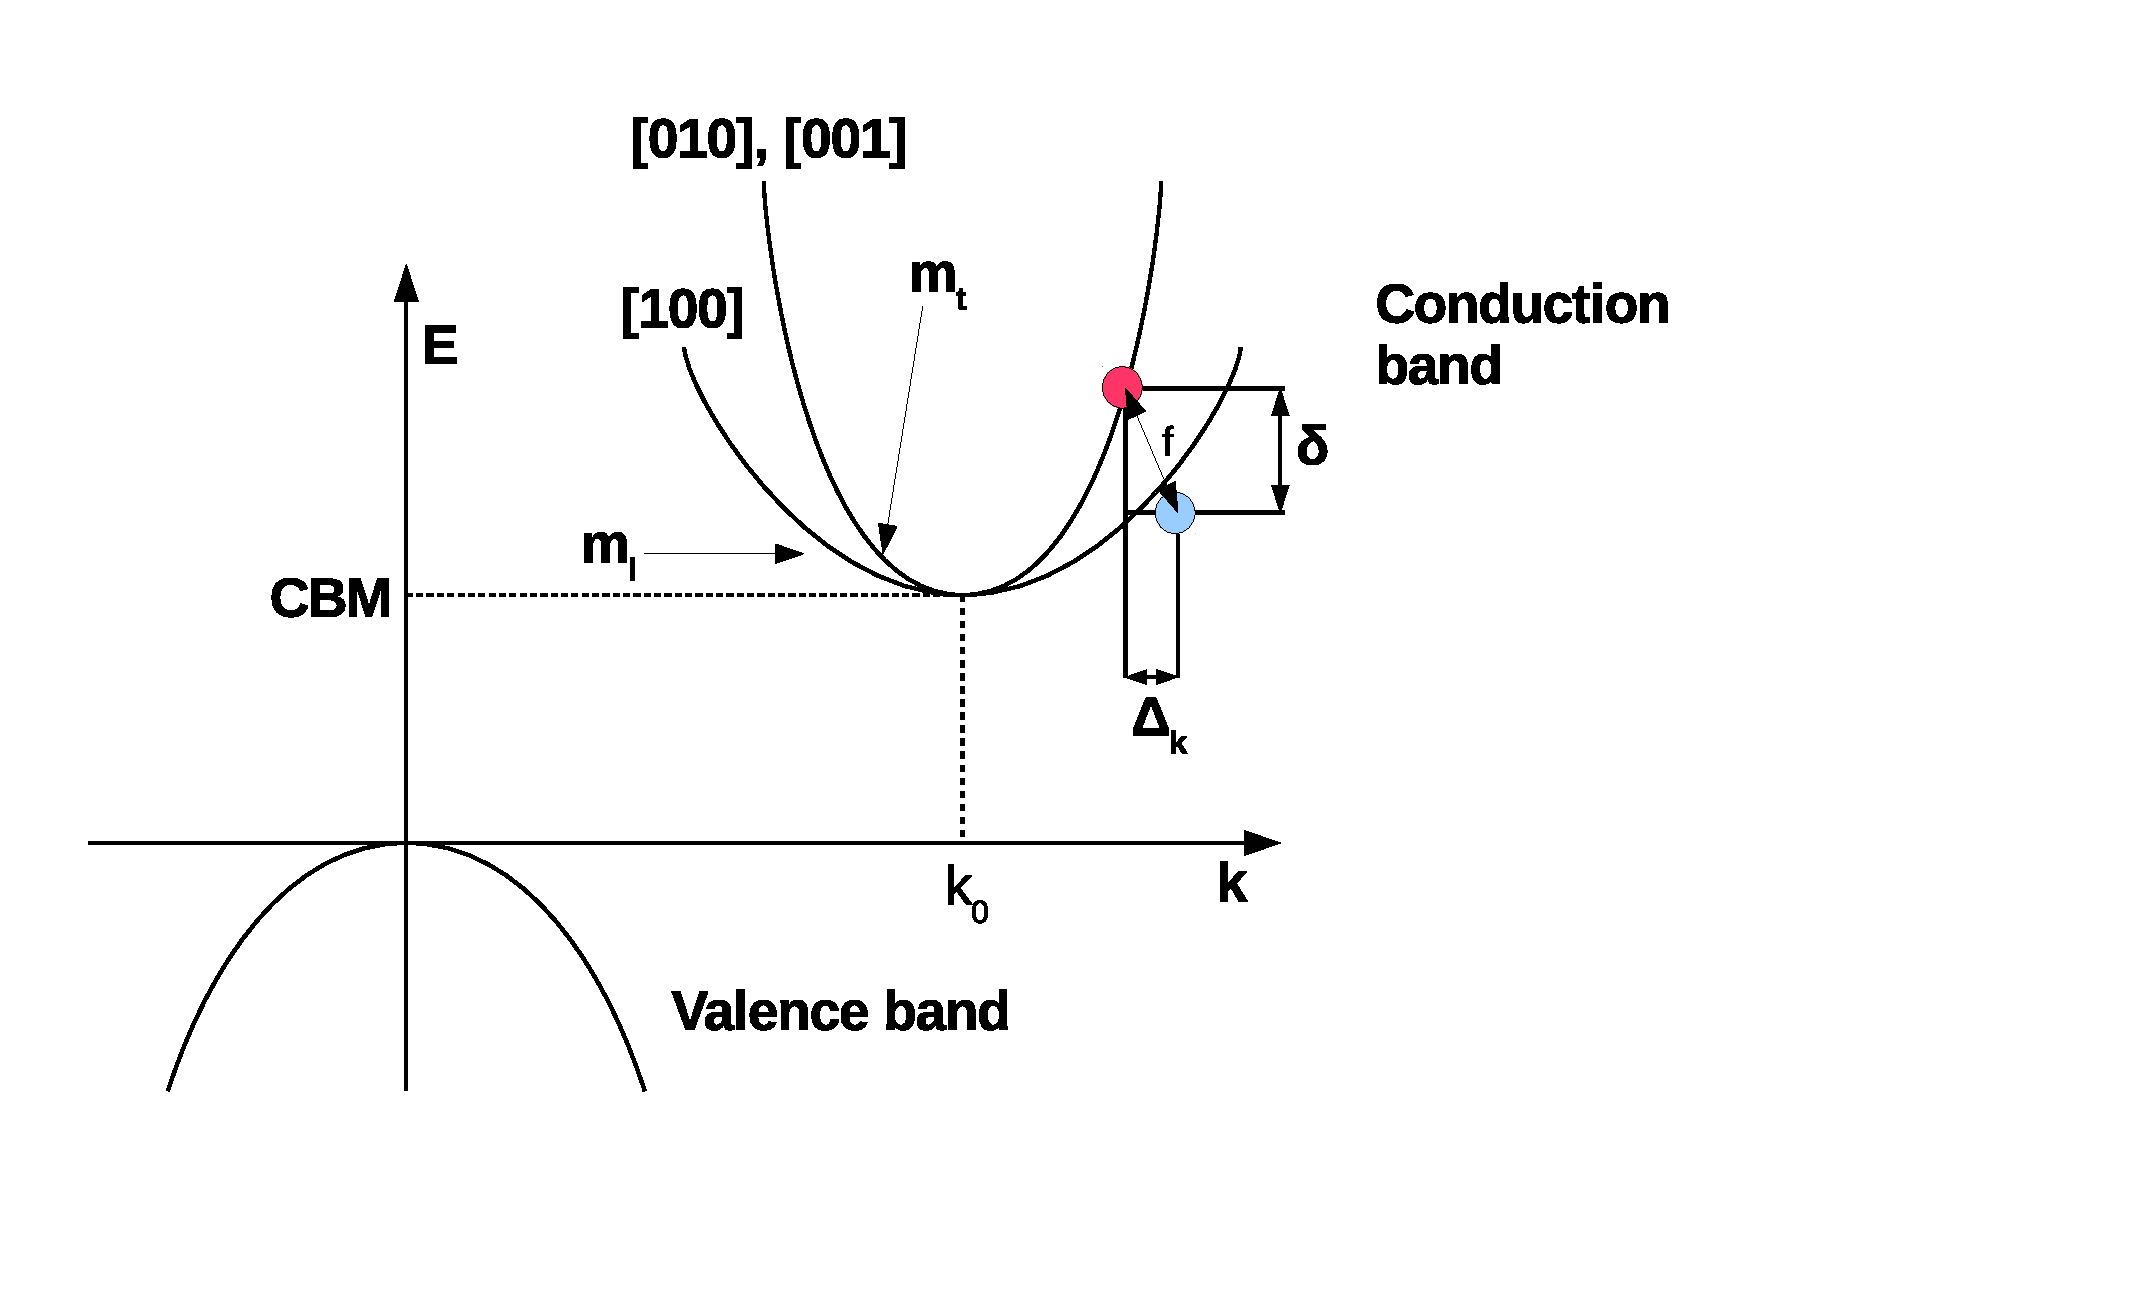
\includegraphics[trim=0 0 50 0, width=0.49\textwidth]{figures/f-scat.eps}
 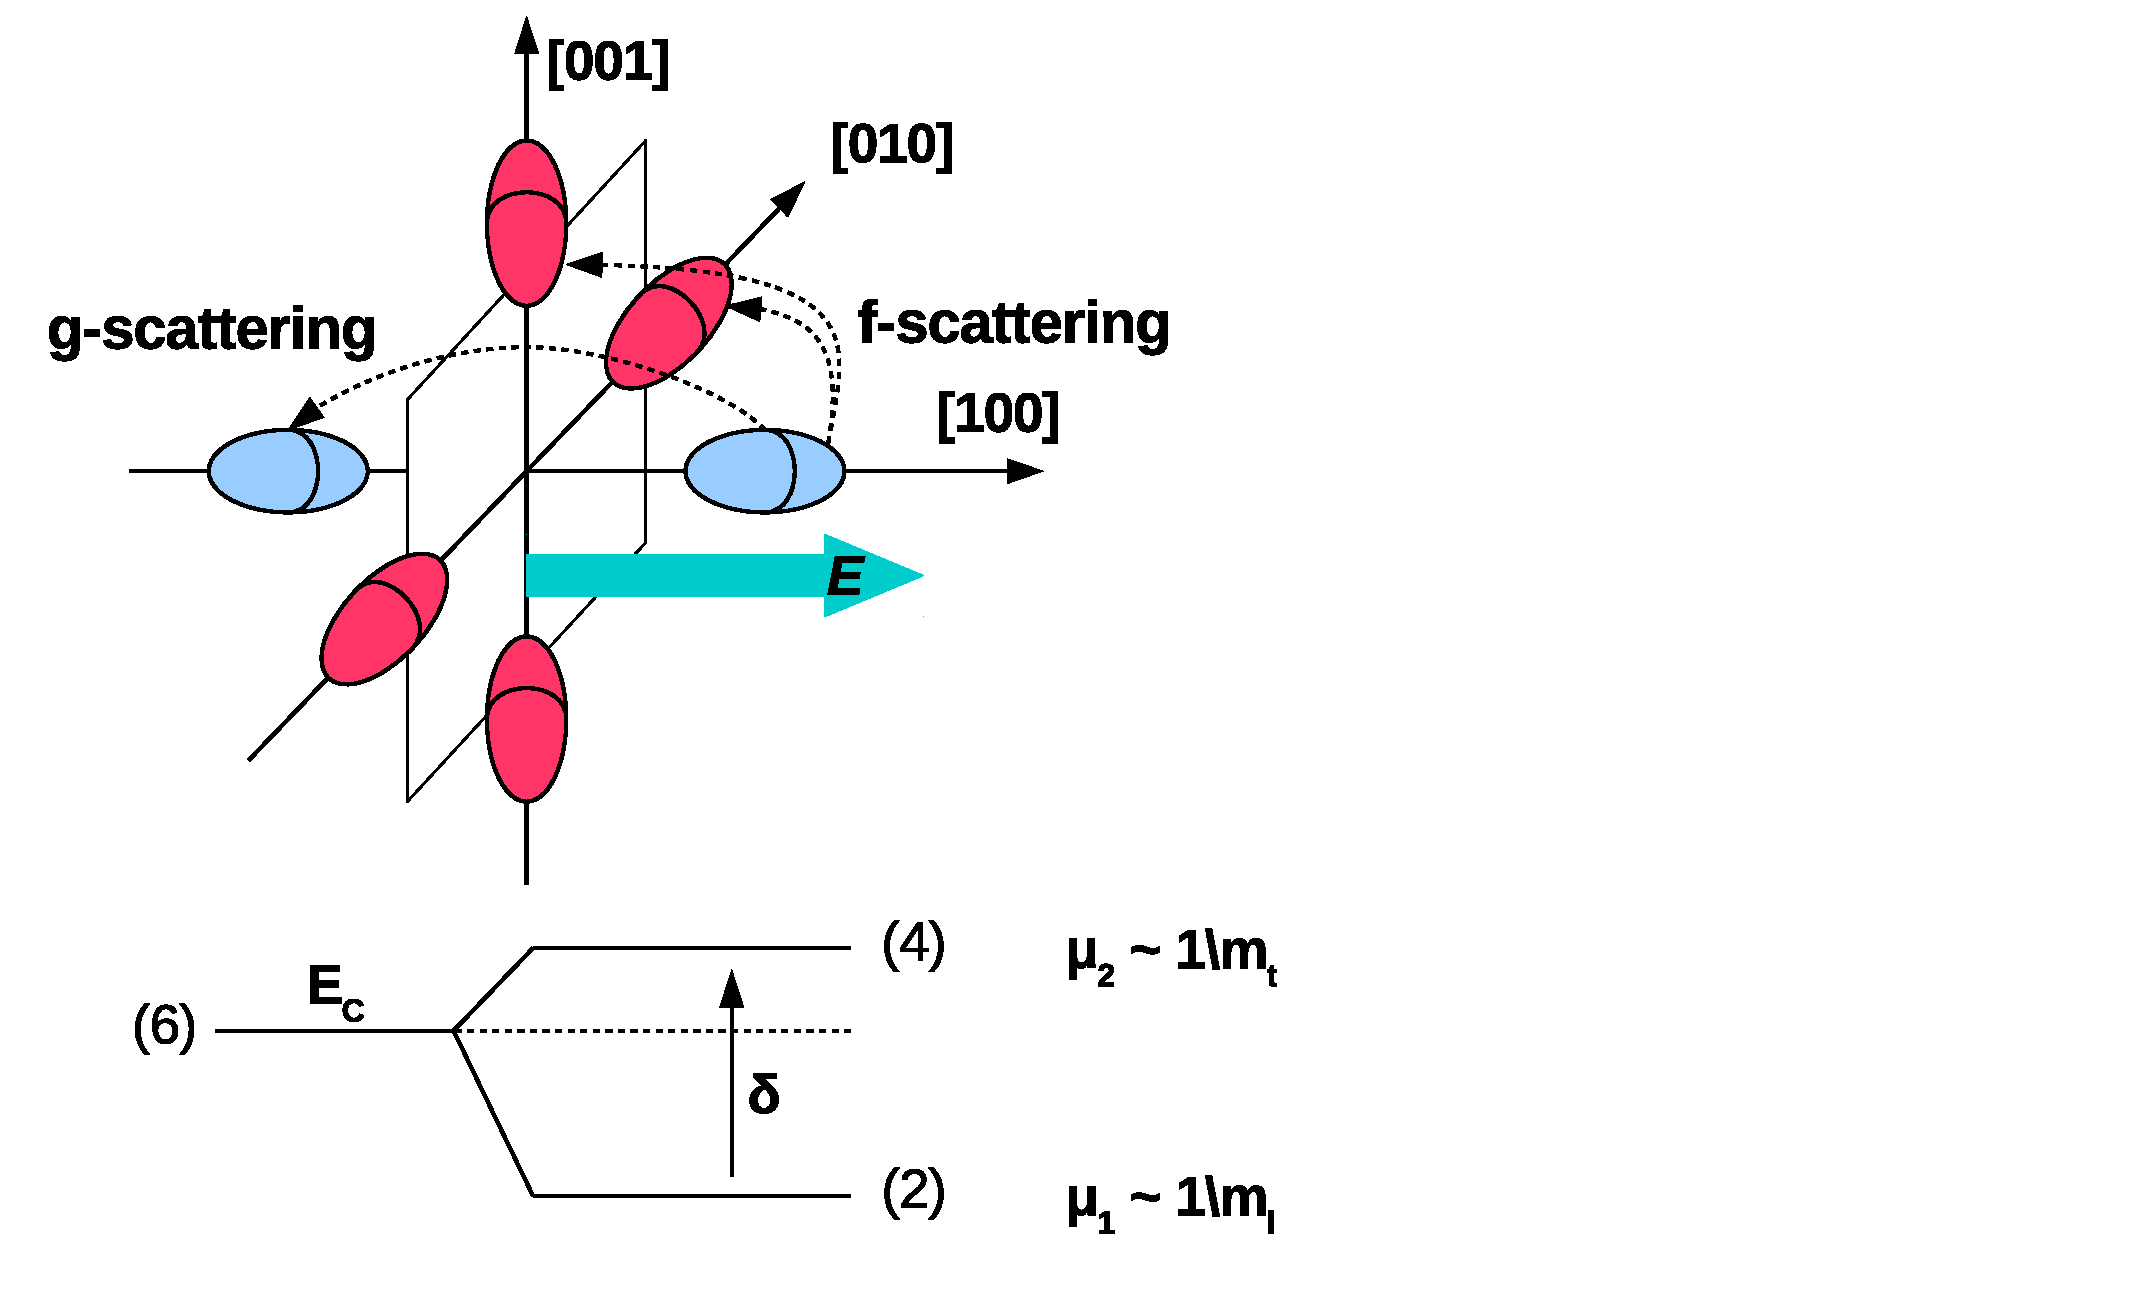
\includegraphics[trim=0 0 50 0, width=0.49\textwidth]{figures/degenerated-states.eps}
 \caption{Shown are the six CBM valleys, which -- under the influence of an electric field -- are two-fold degenerated in the [100] direction and four-fold degenerated in the perpendicular plane. 
 An energy difference $\delta$ characterises the splitting due to the different mass-factors in the dispersion relation. }
 \label{fig:gamma6}
\end{figure}

To explain this effect, we show in Fig.~\ref{fig:gamma6} the orientational valley-orbit splitting of $\Gamma6$ electrons in a homogeneous electric field. 
The electron state splits into two states, one at lower energy with twofold degeneracy for electrons in conduction band valleys parallel to the field direction in $k$-space,
 and the other at higher energy with fourfold degeneracy for electrons in conduction band valleys perpendicular to the field in $k$-space. 
The terms parallel and perpendicular refer to the long  ($\ml$) and short ($\mt$) axes of the valley ellipsoids of constant energy in $k$-space. 
This situation was exhaustively sketched and described in (Ref. \cite{lofas:032139}).

Taking the expression $\mu = \q \tauscat / \mestar$ 
 and assuming equal band scattering times $\tauscat$ in the two substates electrons in the lower state move slowly as their associated effective mass is $\ml = 1.4 \cdot m_0$ 
while electrons in the upper state move fast having a much smaller effective mass $\mt = 0.36\cdot m_0$.

Our situation is different from that studied by Gabrysch et al.\ (Ref.~\cite{isberg:172103,valley,gabrysch:063719} under similar experimental conditions. %FIXME check refs
Their samples are ultra-pure showing extremely little scattering between electrons in the two split substates. 
This enabled them to register the current pulses due to fast and slow electrons individually at different arrival times when reaching the anode. 
From these fascinating experiments they could deduce a firm value for the mass ratio $R = \ml/\mt = 5$. 
This is a much more reliable value than earlier data obtained by less direct methods. 
Such previous values were discussed in Ref.\ ?? and were found as cited above yielding $R = \ml /\mt = 3.9$. 
Our present samples are yellowish {\color{red}(B20)}
 indicating a rather high concentration of nitrogen (deep) donors and possibly other defects causing high scattering rates between the two split states. 
We call the effect which we observe “valley re-population” among the two states,
 and comparison with the samples used by Gabrysch et al.\ demonstrates that it must be induced by impurity-assisted intervalley scattering.

We discuss impurity-assisted scattering in more detail. 
In diamond, the valleys are centred in $k$-space at 0.76 \% of the Brillouin zone at $2\pi/a_0$  in  [100]-type directions. 
Re-population of the two inequivalent parallel and perpendicular valleys means f-type intervalley scattering (IVS) by phonons with suitable wave-vectors $k\, ||\,  [110]$  in $k$-space. 
In a pure crystal, IVS depends on the availability of phonons satisfying the wave-vector and energy conservation rules as well.  
Phonons which can scatter must therefore gap a wave-vector difference of $\Delta k = \sqrt{2}\cdot 0.76 (2\pi/a_0) = 1.07 (2\pi/a_0)$. 
In the  [110]-direction, this is nearly exactly the full length of the Brillouin zone from $k = 0$ ($Γ$-point) to the $K$-point. 
The minimum energy needed for a phonon with this $k$-value is 95\,meV according to the phonon dispersion curves (Ref.\ ??). 
Selection rules may impose further restrictive conditions. 
Unless the two substates are split by this amount there will be no IVS.  
Actually, the electrons have kinetic energy in their valleys so that the cited values of $\Delta k$ and the minimum phonon energy have to be slightly reconciled. 
The samples of the present study contain a significant concentration of defects (e.g.\ nitrogen is a deep donor-like defect) which can take up $k$-vectors
 by virtue of their wave function which is widely spread in $k$-space. 
This invalidates the $k$-conservation rule and enables re-population of the electrons at any splitting.

Experimental proof of impurity-assisted IVS has previously been demonstrated in silicon. 
There, FE and EHD luminescence was studied under uniaxial stress splitting the electron states completely analogously to an electric field,
 and “hot” and “cold” recombination lines were observed due to the electrons in the split upper or lower energy valleys, respectively. 
When the crystals were pure there was no thermalisation of the hot luminescence line at all until the splitting energy reached the TA-phonon energy
 at the adequate scattering wave-vektor $\Delta k\,||\, [110]$ setting then the valley populations into quasi-thermal equilibrium. 
For moderately increased doping with donors or acceptors the hot luminescence line disappeared in succession faster at much lower stress and could no more be observed for high doping levels.

Our present situation can be modelled in a straight forward simple way:  
For strong scattering the population ratio of the two states can be written as a Boltzmann factor in quasi-thermal equilibrium
 
\begin{equation}
 \frac{\nt}{\nl} = \frac{4}{2}\exp{(-\delta/\kB T)}
\end{equation}

\noindent
with the splitting energy $\delta$ and {\color{red}(B21)}

\begin{equation}
 \nt = \frac{N}{1+2\exp{(-\delta/\kB T)}}, \qquad  \nl = \frac{N}{1+1/2\exp{(-\delta/\kB T)}},
\end{equation}

\noindent
where $N = \nt + \nl$ is the concentration of electrons in both states. 
The total current amounts to  {\color{red}(B22)}

\begin{equation}
 j = j_{\textrm{t}} + j_{\textrm{l}} = \q\left( \nt \vt + \nl \vl \right) = \q N \xi \left( \frac{\mut}{1+2\exp{(-\delta/\kB T)}}  + \frac{\mul}{1+1/2\exp{(+\delta/\kB T)}}\right) 
\end{equation}

\noindent
using $v_{\textrm{t/l}} = \mu_{\textrm{t/l}}\xi$. 
After some reformulation {\color{red}(B23)} we find for the transit time

\begin{equation}
 t' = \frac{d}{\mul\xi}\cdot \frac{1}{ \dfrac{1}{1+2\exp{(-\delta/\kB T)}}\cdot(1-R) + R} \quad {\color{red}(B23')}.
 \label{math:tprime}
\end{equation}

We have still to associate the splitting energies $\delta$ with the applied voltages. 
To this sake it is important to note that $\delta$ is not primarily due to an electrostatic splitting which is estimated to amount to only a few meV at the highest field strengths. 
Owing to lacking literature data on the electric compliance constants we cannot calculate such values. 
Instead, we are concerned with a dynamic splitting due to the kinetic energy of the electrons when moving in the two states. 
With $E_{\textrm{kin,t/l}} = 1/2 m_{\e,\textrm{t/l}}v_{\textrm{t/l}}^2$, we find {\color{red}(B24)}

\begin{equation}
 \delta = \Delta E_{\textrm{kin}} = 1/2 \cdot\ml \vl^2 - 1/2 \cdot\mt \vt^2.
\end{equation}

\noindent
Using the above cited mass ratio $R =5$ results in

\begin{equation}
 \delta = 2 \ml \vl^2
\end{equation}

\noindent
There is no accurate analytic expression for $\vdrift$ as a function of $\xi$ or the applied voltage,
 but numerical values $\vdrift(\xi)$ can be extracted from experimental data in reference \cite{jansen:173706} in Fig.~5 (b). 
Some values are explicitly quoted in table~\ref{tab:deltas} {\color{red}(B25)}.
In this compilation, a value of $\ml  = 1.36\,m_0$  was used {\color{red}(B26)}.

\begin{table}[t]
\caption[delta values]{Compilation of extracted values of $\vdrift$ and $\delta$.}
 \begin{center}
  \begin{tabular}{c|c|c||c|c|c||c|c}
  voltage $U$ & $\vdrift$ & $\delta$ & v at RT& v(225\,K) & v(150\,K) & $\delta$ (150\,K) & $\vl$(150\,K)\\
  $[\si{\volt}]$  & $[10^4\,\si{\m/\s}]$  & $[\si{\meV}]$  &  $[10^6\,\si{\cm/\s}]$ &  & & $[\si{\meV}]$  & $[10^4\,\si{\m/\s}]$\\ \hline
  40  &      &       & 1.5  & 2.1 &  1.9 & &\\
  60  & 3.2  &  15.8 & 2.0  & 2.5 &  2.1 &   1.0 &  0.58\\
  80  & 4.0  &  24.7 & 2.5  & 2.9 &  2.3 & &  \\
  100 & 4.6  &  32.6 & 2.8  & 3.1 &  2.7 &   1.7 &  0.75\\
  150 & 5.9  &  53.8 & 3.6  & 3.6 &  3.8 & &  \\
  200 & 7.0  &  75.7 & 4.2  & 4.2 &  4.8 &   5.9 &  1.4\\
  300 &      &       & 5.0  & 5.3 &  6.3 &  11.6 &  1.9\\
  400 & 9.5  & 139.0 & 5.6  & 6.3 &  7.4 & 165   &  7.3\\
  500 & 10.2 & 160.2 & 6.3  & 7.0 &  8.3 & 212   &  8.3\\
  900 &      &       & 8.2  & 9.2 & 10.3 & 328   & 10.3\\
  \end{tabular}
  \label{tab:deltas}
 \end{center}
\end{table}

\begin{figure}[tb]
 \centering
 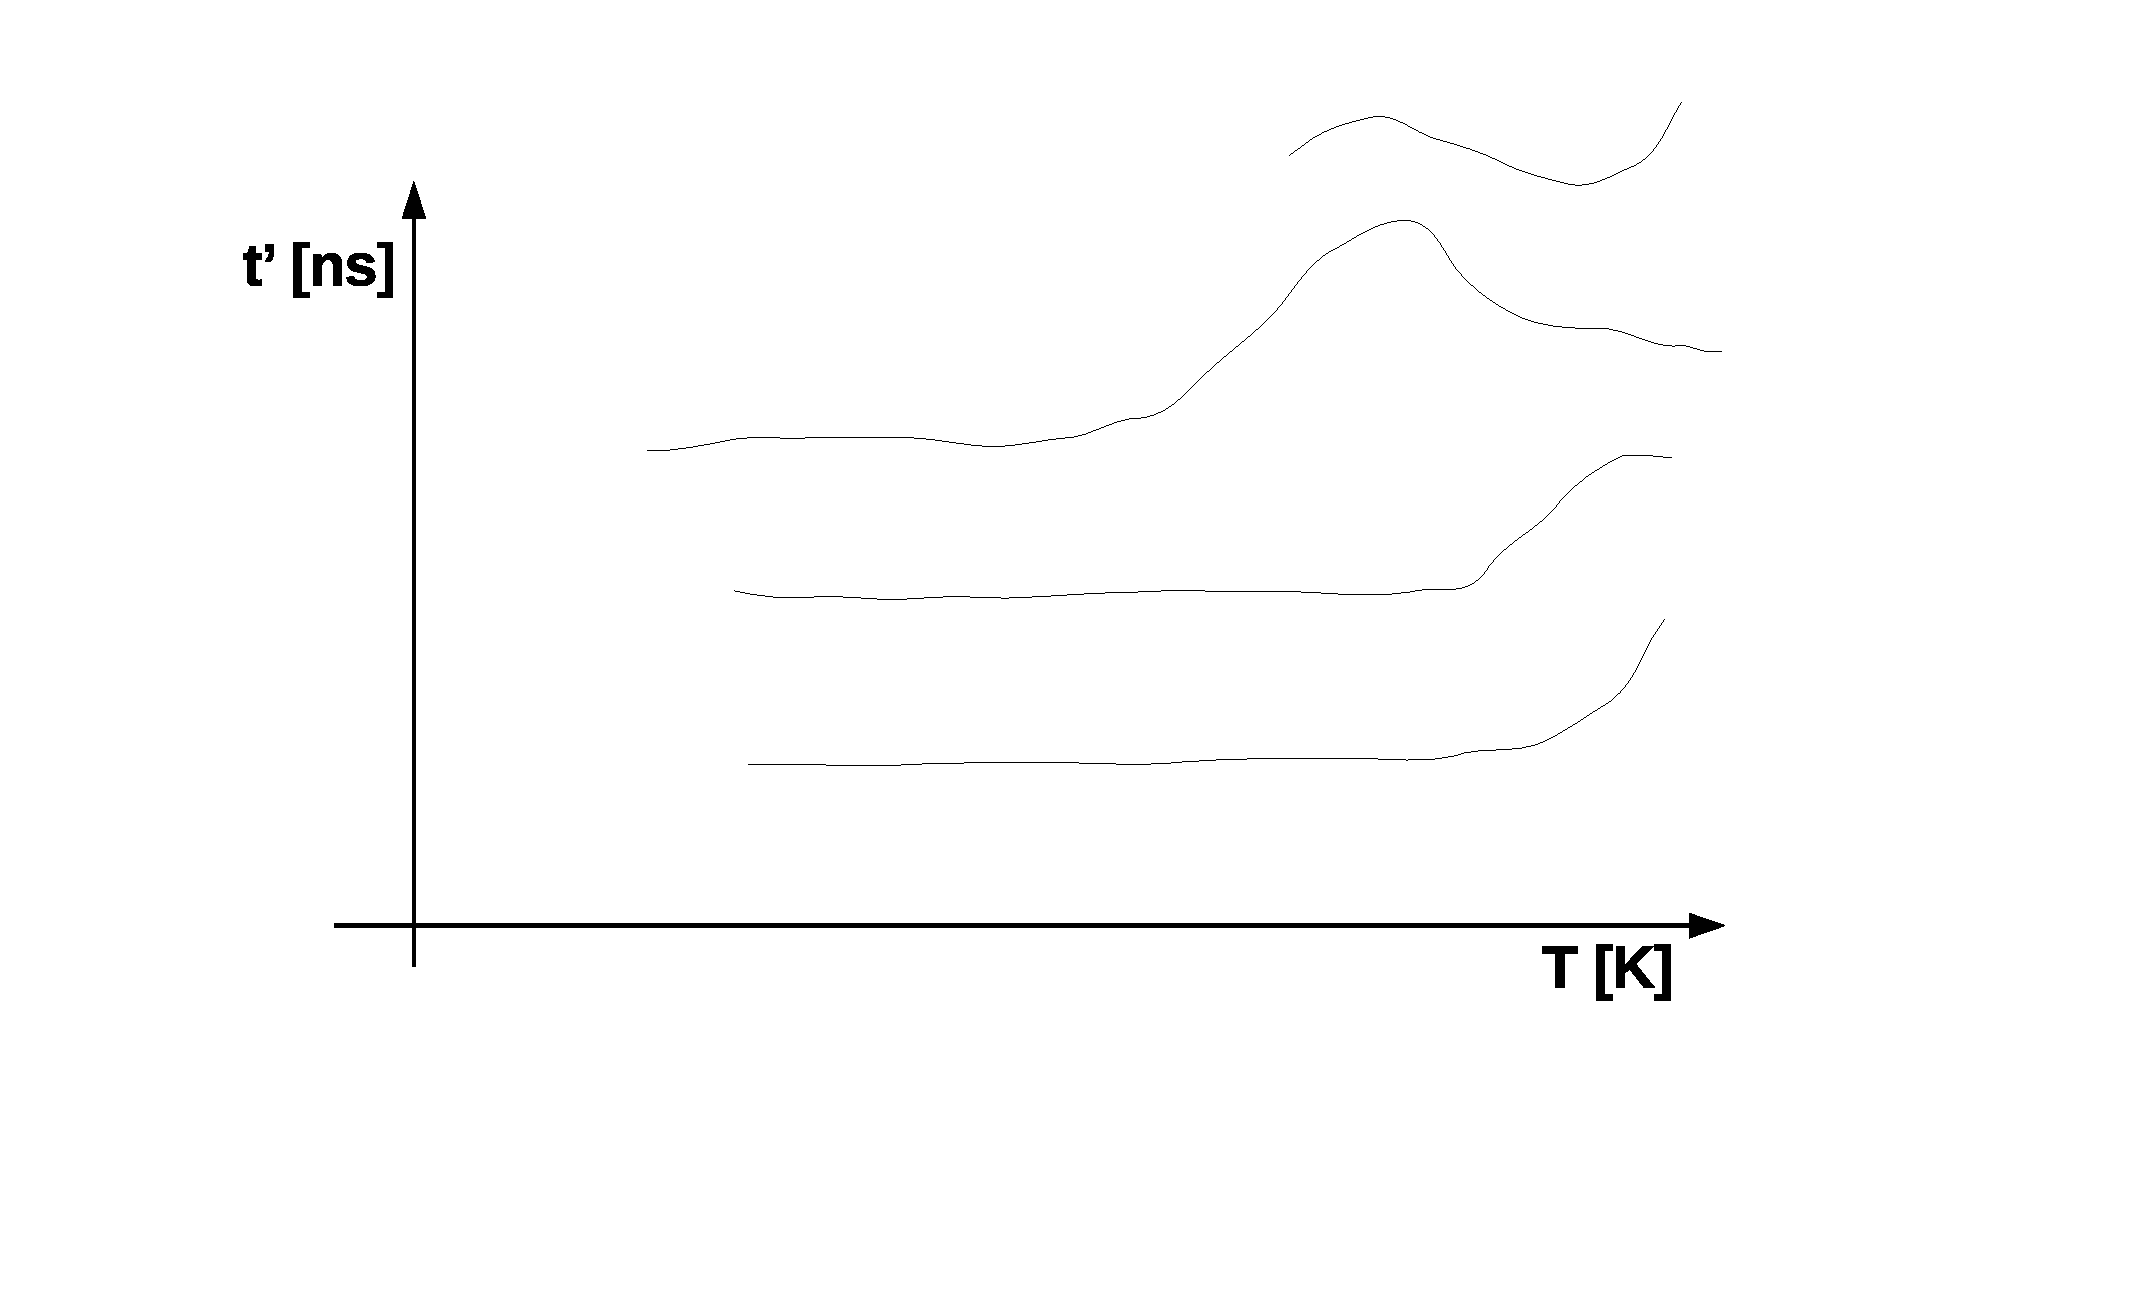
\includegraphics[trim=0 150 0 0, width=0.80\textwidth]{figures/dummy_repop.eps}
 \caption{Siehe Anmerkungen {\color{red}(B27)}}
 \label{fig:repop}
\end{figure}


For the model curves represented in Fig.~\ref{fig:repop}  the transit time was taken in the alternative form {\color{red}(B27)}

\begin{equation}
 t' = \frac{\SI{500}{\um}}{\vl}\frac{1+2\exp{(-\delta/\kB T)}}{1+10\exp{(-\delta/\kB T)}} \equiv \frac{\SI{500}{\um}}{v_{\textrm{eff}}}
\end{equation}

\noindent
following from equation (\ref{math:tprime}) after inserting $R = 5$, and $\vl$ was numerically associated with the applied voltages according to table~\ref{tab:deltas}.
To account for the basic phonon scattering as a function of temperature underlying all experimental curves in Fig.~\ref{fig:tt}, we have employed the entirely empirical expression {\color{red}(B28)}

\begin{equation}
 t_{\textrm{basic}} = \left( 4.3 - \num{0.6e-4}\,T + \num{2.2e-5}\,T^2 \right) \cdot \frac{500}{U} ^{\left( 0.5 + \frac{0.6}{300\,T} \right)} \textrm{ in nanoseconds}.
\end{equation}

\noindent
Comparison of these model curves with the measured curves (Fig.~\ref{fig:repop}) {\color{red}(B27)} shows that the model reproduces all relevant characteristic aspects in a convincing way. 
In detail, however, there is no satisfactory quantitative agreement. 
This may be due to the mass value chosen, deviations from a parabolic band dispersion which we have tacitly implied by the form of the kinetic energy and which can become crucial for the high energies involved,
 neglect of the static splitting of the substates, or numerical uncertainties in the listing given above.


